%%%%%%%%%%%%%%%%%%%%%%%%%%%%%%%%%%%%%%%%%
% Arsclassica Article
% LaTeX Template
% Version 1.1 (10/6/14)
%
% This template has been downloaded from:
% http://www.LaTeXTemplates.com
%
% Original author:
% Lorenzo Pantieri (http://www.lorenzopantieri.net) with extensive modifications by:
% Vel (vel@latextemplates.com)
%
% License:
% CC BY-NC-SA 3.0 (http://creativecommons.org/licenses/by-nc-sa/3.0/)
%
%%%%%%%%%%%%%%%%%%%%%%%%%%%%%%%%%%%%%%%%%

%----------------------------------------------------------------------------------------
%	PACKAGES AND OTHER DOCUMENT CONFIGURATIONS
%----------------------------------------------------------------------------------------

\documentclass[
10pt, % Main document font size
a4paper, % Paper type, use 'letterpaper' for US Letter paper
oneside, % One page layout (no page indentation)
%twoside, % Two page layout (page indentation for binding and different headers)
headinclude,footinclude, % Extra spacing for the header and footer
BCOR5mm, % Binding correction
]{scrartcl}

\input{structure.tex} % Include the structure.tex file which specified the document structure and layout

\hyphenation{Fortran hy-phen-ation} % Specify custom hyphenation points in words with dashes where you would like hyphenation to occur, or alternatively, don't put any dashes in a word to stop hyphenation altogether

%% additional packages:
\usepackage{wrapfig}
\usepackage[left=1in,right=1in,top=1in,bottom=1in]{geometry}
\usepackage{caption}

%----------------------------------------------------------------------------------------
%	TITLE AND AUTHOR(S)
%----------------------------------------------------------------------------------------

\title{ \vspace{-3em}

\includegraphics[width=.1\textwidth]{Figures/logo.png} \\
\includegraphics[width=4cm]{Figures/logotext.png} \\
} % The article title

\author{  Summer data challenge entry by Benjamin
  L. Moore\textsuperscript{1} } % The article author(s) - author affiliations need to be specified in the AUTHOR AFFILIATIONS block

\date{} % An optional date to appear under the author(s)

%----------------------------------------------------------------------------------------

% custom macros:

\newcommand*{\logo}{\includegraphics[scale=.04]{Figures/logotext.png}}

\begin{document}

%----------------------------------------------------------------------------------------
%	HEADERS
%----------------------------------------------------------------------------------------

%\renewcommand{\sectionmark}[1]{
\markright{\spacedlowsmallcaps{summerdatachallenge}}
%} % The header for all pages (oneside) or for even pages (twoside)
%\renewcommand{\subsectionmark}[1]{\markright{\thesubsection~#1}} % Uncomment when using the twoside option - this modifies the header on odd pages
\lehead{\mbox{\llap{\small\thepage\kern1em\color{halfgray} \vline}\color{halfgray}\hspace{0.5em}\rightmark\hfil}} % The header style

\pagestyle{scrheadings} % Enable the headers specified in this block

%----------------------------------------------------------------------------------------
%	TABLE OF CONTENTS & LISTS OF FIGURES AND TABLES
%----------------------------------------------------------------------------------------

% \maketitle % Print the title/author/date block

\setcounter{tocdepth}{2} % Set the depth of the table of contents to show sections and subsections only

% \tableofcontents % Print the table of contents

% \listoffigures % Print the list of figures

% \listoftables % Print the list of tables

% Make header in inkscape?
\begin{figure}[width=\textwidth]
\vspace{-3em}
\centering
\includegraphics[width=.7\textwidth]{Figures/header2.pdf}
\vspace{.5em}
\end{figure}

%suppres headers
\thispagestyle{plain}

%----------------------------------------------------------------------------------------
%	ABSTRACT
%----------------------------------------------------------------------------------------
\vspace{-4em}
\section*{Overview} 

\setlength{\intextsep}{0em}
\begin{wrapfigure}{R}{.3\textwidth}
%\vspace{-1em}
\centering
\includegraphics[width=.28\textwidth]{Figures/overview.png}
\vspace{-1em}
\caption*{ A map of the house prices dataset (brightness is proportional to
  price and density).}
\end{wrapfigure}

I analysed the {\bf London house prices} dataset in several innovative
ways. Firstly \emph{fractal context} shows how house sales within an
arbitrary area relate to those if neighbouring districs, up and down
the postcode hierarchy. Secondly, I fit \emph{ARIMA models} to
forecast an area's price trend into the future, with an eye to
suggesting profitable investments. Finally, these and other metrics
were combined into an \emph{investment grade} for a given postcode
area. Together this set of analyses forms the basis of \logo, a
startup aimed at \emph{democratising real estate investment}, offering
individuals and businesses quantitative property area insights to enable
data-driven investment decisions.

A full report with additional interactive visualisations is online at {\bf
  \leavevmode\href{http://blm.io/datarea}{blm.io/datarea} }and scripts to
reproduce all analyses are available from {\bf
  \leavevmode\href{http://github.com/blmoore/summerdatachallenge}{github.com/blmoore/summerdatachallenge}}.

%----------------------------------------------------------------------------------------
%	AUTHOR AFFILIATIONS
%----------------------------------------------------------------------------------------

{\let\thefootnote\relax\footnotetext{\textsuperscript{1} \textit{MRC
      Human Genetics Unit, University of Edinburgh, Scotland, United Kingdom}}}

%----------------------------------------------------------------------------------------

%\newpage % Start the article content on the second page, remove this if you have a longer abstract that goes onto the second page

%----------------------------------------------------------------------------------------
%	INTRODUCTION
%----------------------------------------------------------------------------------------

\vspace{-1em}
\section*{Section A: Analyses}

When considering a property in a given area, you may ask a realtor
questions like: how do prices here compare to surrounding postcodes, and
how have they changed over time? A real estate professional can
give an opinion based on their own limited sample size, but with a
large dataset we can address these questions quantitatively and
visualise the results.

\vspace{-.5em}
\subsection*{Fractal context}

Letting and sales sites may currently list some recent sales, but it's
not currently possible to see a quantitative overview of property
prices in a region, within the context of its sector, district and
postcode.

%\setlength{\intextsep}{0em}
\begin{wrapfigure}[16]{l}{.45\textwidth}
\vspace{.5em}
\centering
\includegraphics[width=.43\textwidth]{Figures/fractal.png}
\caption{ Fractal context of postcode SW18 4HU in Wandsworth, South London.}
%\vspace{35em}
\end{wrapfigure}

%\noindent 

These questions can be answered with a clear and intuitive data
visualisation of price distributions in the postcode hierarchy --- we
call this the fractal context of a property price (Figure 1).

A specific postcode or area can be marked within its distribution,
giving a clear view of a properties relative pricing which cannot be
gleaned just by browsing recent sales. The example view (Figure 1)
combines ranked violin density plots and a geo-heatmap for a clear,
intuitive view of a locations price context.

\vspace{-.5em}
\subsection*{ARIMA modelling}

Given a time series of housing prices, it's of interest to investors
to speculate on potential investment returns for a given property
area. This can be done through time series analysis using the
autoregressive integrated moving average (ARIMA) model (Figure 2). The
model fitting procedure included regularisation that allowed a $drift$
term to model non-stationary trends, as well as coefficients capturing
periodicity or seasonal effects. Potential investment returns could be
optimised by selecting areas with
maximal growth projections. \\

\begin{figure}[h]
\begin{center}
\includegraphics[width=.9\textwidth]{Figures/arima.png}
\caption{Example ARIMA forecast of median house prices for a specific postcode.}
\end{center}
\end{figure}

\vspace{-2em}
\subsection*{Investment grading}

Combining growth forecasts and other derived metrics from this
dataset allow an approximate investment grading, relative to other
postcodes within the area covered by this dataset. This intuitive
output metric can help prioritise areas ripe for property investment.

As an example, Figure 3 shows the top 5 postcode sectors
in which to invest, according to their 12-month price growth forecast
and historical annualised volatility --- thus combining the empirical
data with theoretical model outputs. These include Brockley,
whose train station within SE4 1 was linked with the London Overground network in 2010.\\

\begin{figure}[h]
\begin{center}
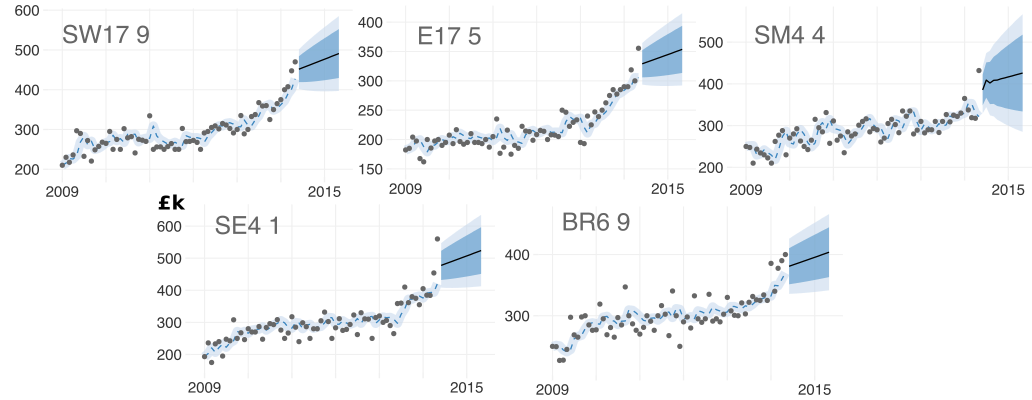
\includegraphics[width=.9\textwidth]{Figures/t5.pdf}
\caption{Top 5 property investment sectors by projected returns and historical volatility.}
\end{center}
\end{figure}

\setlength{\intextsep}{0em}
\begin{wrapfigure}{R}{.45\textwidth}
\vspace{.5em}
\centering
\includegraphics[width=.44\textwidth]{inkscape/grading_2.png}
\vspace{-1em}
\caption{ Quantile transformation for investment grading
  (AAA rated sectors in \emph{navy}).}
\vspace{.5em}
\end{wrapfigure}

Growth forecasts and volatility were converted to quantiles and
weighted equally; those sectors with the highest projected growth
and least historical volatility receive the best investment grade
(on a scale of AAA, AA, A, BBB \ldots C).\textsuperscript{$\star$}

Returning to our original example, SW18 4HU is a promising choice of
area for property investment. It's median-priced for the sector, which
is the cheapest of SW18 (in turn part of the desirable SW London area;
Figure 1). It has good growth projections of over £28,000 in the next
year (Figure 2), and receives the top AAA investment grade, being
in the 90\textsuperscript{th} percentile for predicted price growth
and low historical volatility in the dataset.

{\let\thefootnote\relax\footnotetext{\textsuperscript{$\star$}
    Data intended to assist investors and does not constitute
    investment advice; independent advice should be sought where appropriate. }}

%----------------------------------------------------------------------------------------
%	METHODS
%----------------------------------------------------------------------------------------
\clearpage
\section*{Section B: Value generation}

The above-described analyses form the basis of \logo\hspace{.1em}, a
start-up aimed at ``democratising real estate investment'' by making
deep-dive analytics data available both to a consumer and professional
investment market. Initially \logo\hspace{.1em} is a provider of
information aimed at investors but cannot dispense investment advice
until authorised to do so by the FCA. Three initial areas of interest
to commercialise and generate social and economic value are listed:

\subsection*{1. Analytics provider for online house sales and lettings
agents}

\logo\hspace{.1em} can provide {\bf real-time property area analytics} to
existing market leaders in {\bf online sales and lettings}. 

\begin{wrapfigure}{l}{.25\textwidth}
\begin{center}
\includegraphics[width=.18\textwidth]{Figures/zoopla.png}
\includegraphics[width=.23\textwidth]{Figures/rightmove.jpg}
\caption*{ Potential partners. }
\end{center}
\end{wrapfigure}

There are currently no mainsteam property sales or rental sites that
attempts to provide any quantitative insights to contextualise a
property's list price. Some list recent nearby sales in plain text,
but the wealth of historical sales data available allows for much
richer displays (as demonstrated with the fractal context view,
\emph{above}), which offer valuable and practical insights to
prospective homebuyers.

This added feature would help differentiate a given sales and letting
site as well as increase the brand positioning of \logo\hspace{.1em}
within the real estate sector. Contextual maps could be drawn as
interactive D3.js visualisations and neatly integrated with a typical
property search. Additionally, web analytics data from our partnered
site could be fed-back to help further enhancement and expansion of
the data-driven insights and visualisations we offer.

\begin{figure}[h]
\vspace{1.5em}
\centering
\includegraphics[width=.85\textwidth]{Figures/gmapScreenshot.png}
\vspace{.5em}
\caption{ A basic embeddable web app built with the Google Maps API
  (viewable at \href{http://blm.io/datarea}{blm.io/datarea}). }
\end{figure}

\subsection*{2. Direct-to-consumer demo application}

\logo \hspace{.1em} would release both a {\bf web service} and associated
{\bf mobiles and tablet applications}. These would offer limited analysis and
visualisation without any fee, with collected user data and feedback helping to
validate the business model and develop our software.

\begin{wrapfigure}[12]{r}{.4\textwidth}
\centering
\includegraphics[width=.39\textwidth]{Figures/mockup.png}
\caption{ iOS app mock-up.}
%\vspace{-1em}
\end{wrapfigure}

Releasing these products aligns with our aims of democratising real
estate investment. Amateur property investors and prospective
landlords can make data-driven decisions, the likes of which are likely
already employed by large investment trusts and funds. 

A small data science team will gradually expand the range of analyses
offered, integrating novel public and privately-acquired datasets and
release them under a rolling subscription model, aimed at private
landlords and property speculators, as well as professional real
estate investment trusts (REITs). Significant revenue could be
generated through tailored partnerships with funds and high net-worth
individuals.

\subsection*{3. Real estate data science consultancy}

Having established a property area analytics brand, \logo\hspace{.1em}
will look to develop business relationships with real estate
investment funds and high net-worth individuals as a {\bf quantitative
  property investment consultancy} and independent analyst for the
financial services. Our domain expertise and existing partnerships and
products would place us as a market leader in this undeveloped
segment.

\section*{Summary}

\begin{wrapfigure}[10]{r}{.3\textwidth}
\vspace{2em}
\centering

\includegraphics[width=.2\textwidth]{Figures/logo.png}
\includegraphics[width=.2\textwidth]{Figures/logotext.png}
%\caption*{ {\sf Democratising real estate investment}}
\caption{ Logo design. }
%\vspace{-4em}
\end{wrapfigure}

In this report I've given a brief overview my attempts to elute
maximal insight from a single large dataset through visualisations and
quantitative modelling. Together these form a cohesive narrative of
investigative analysis into a single exemplar postcode, and discovery
of the potential investment returns therein.

These analyses have the potential to generate valuable insights for a range of
customer segments:
\begin{itemize}

\item Online sales and letting agents would benefit from
plug-in analytics provided by \logo \hspace{.1em} --- offering their
users advanced insights into spatiotemporal property statistics.

\item A web and mobile app to make a set of analyses widely-available
  to amateur property investors, new homebuyers and landlords.

\item A consultancy specialising in real estate investment to partner
  with REITs and other specialist investment funds, as well as
  charitable trusts.
\end{itemize}

\vspace{1em}
\begin{flushright} {\small An enhanced online version of this short
    report is available at:
    \leavevmode\href{http://blm.io/datarea}{blm.io/datarea}}
\end{flushright}

%\vspace{2em}
% \begin{figure}[h!]
% \begin{center}
% 
\includegraphics[width=.15\textwidth]{Figures/logo.png} \\
% \includegraphics[scale=.11]{Figures/logotext.png} \\
% \caption*{ {\sf Democratising real estate investment}}
% \end{center}
% \end{figure}

\end{document}